
\documentclass[submit]{ipsj}
%\documentclass{ipsj}

% \usepackage{graphicx}
\usepackage[dvipdfmx]{graphicx}
\usepackage{latexsym}

\def\Underline{\setbox0\hbox\bgroup\let\\\endUnderline}
\def\endUnderline{\vphantom{y}\egroup\smash{\underline{\box0}}\\}
\def\|{\verb|}

\setcounter{巻数}{1}
\setcounter{号数}{1}
\setcounter{page}{1}


\受付{2016}{3}{4}
\再受付{2015}{7}{16}   %省略可能
\再再受付{2015}{7}{20} %省略可能
\再再受付{2015}{11}{20} %省略可能
\採録{2016}{8}{1}


\begin{document}


% \title{ユーザの既訪問スポットの位置付けに基づく\\未訪問スポットの説明手法}
\title{ユーザレビューを用いたスポット対応付け手法の\\提案とその応用}

% \etitle{An Explanation Method of Unfamiliar Tourist Spots based on Roles of User's Familiar Spots}
\etitle{Proposal of Spot Matching Method Using User Review And Its Application}

% \affiliate{IPSJ}{情報処理学会\\
% IPSJ, Chiyoda, Tokyo 101--0062, Japan}

\affiliate{Uni}{工学院大学\\Kogakuin Uniersity}

\author{潘 健太}{Han Kenta}{Uni}[em18011@ns.kogakuin.ac.jp]
\author{北山 大輔}{Kitayama Daisuke Hanako}{Uni}[kitayama@cc.kogakuin.ac.jp]

\begin{abstract}
近年,ユーザはWeb上の観光情報を活用して旅行計画を立てることが多くなっている.
しかし,旅行は未訪問スポットに行くことが多いため,観光情報を適切に入手することは困難である.
また,ユーザの未知なスポットに対する理解を支援するために,訪問したことがある観光スポットの特徴を用いて,未訪問エリアの観光スポットを説明する方法を提案する.
本研究では,まず,観光スポットのユーザレビューを用いて特徴ベクトルを作成する.
次に,ユーザにとっての観光スポットの位置付けを抽出するためにあるスポットに対し,既に訪れたスポットと比較した相対的特徴ベクトルを算出する.
最後に,相対的特徴ベクトル間の類似度に基づいて既訪問スポットと未訪問スポットを関連付けし,その関係性を説明するためのキーワードを抽出する.
また,プロトタイプシステムを構築し,既訪問スポットと未訪問スポットとの説明情報の効果を検証する評価実験を行う.
\end{abstract}


\begin{jkeyword}
観光スポット,理解支援,ユーザレビュー,分散表現
\end{jkeyword}

\begin{eabstract}
% 多くの観光客は,レジャー旅行を計画するときに,オンラインから利用可能情報を得ている.しかし,旅行客は未訪問エリアに向けられるかもしれないので,この頼りはしばしば問題を生じそして誤解を招くようになる.
Most tourists resort to available information online when planning for leisure travel; however, this recourse often becomes problematic and misleading as tourist of the information may be directed to unfamiliar areas.
% この点に関して,我々は彼らが既に訪れたことがあるスポットの特徴を通して未訪問スポットを説明する方法を提案した.
On this regard, we proposed a method of explaining unfamiliar spots through the familiar features of spots they have visited.
% 本研究では,まず,観光スポットのユーザレビューを用いて特徴ベクトルを生成した.
In this paper, at first, we generated the feature vector using user reviews of the tourist spot.
% 次に,既に訪問したスポットと比較した相対的な特徴ベクトルを用いて,観光スポットの独特な特徴を抽出した.
Next, we used the relative feature vector compared with already visited spots to extract the role of the tourist spot for the user.
% 最後に,相対的特徴ベクトルの類似性によって訪問スポットを未訪問スポットと関連付け,さらにその関係を説明するキーワードを抽出した.
Finally, we associated the visited spot with the unfamiliar spot by the similarity of the relative feature vector, and further extracted keywords that explain the relation.
% また,システムのプロトタイプを開発し,既訪問スポットと未訪問スポットの間の説明情報の効果を評価した.
Furthermore, we developed a prototype of the system and evaluated the effect of the explanatory information between the familiar and unfamiliar spots.
\end{eabstract}

\begin{ekeyword}
Tourist spots, explainability, tourist reviews, paragraph vector
\end{ekeyword}

\maketitle

%1
\section{はじめに}

旅行先を決定するとき,旅行者は観光スポット検索サイトや観光情報に関連する書籍を見て観光スポットを選び,旅行計画を立てる.
しかし,ユーザにとって訪問したいエリアは,訪問したことがなく不慣れであることが多い.
そのため,エリア内に数多く存在する観光スポットから,自身の要求に合う観光スポットを見つけることは容易ではない.

Tripadvisor\footnote{https://www.tripadvisor.com/}やじゃらん\footnote{https://www.jalan.net/kankou/}などの観光スポット検索サイトでは,特定の観光スポットを訪問したことのあるユーザがレビューを投稿するため,観光スポットに関する豊富な情報が存在している.
これらのレビューサイトは,ユーザの意思決定の材料になりえる.
しかし,ユーザは検索エリアに関する事前知識がないため効率的に読むことは困難である.
そこで我々は,さまざまな観光スポットを効果的に理解するためには,ユーザが訪問した経験のあるスポットを使って未訪問スポットと比較できることが重要であると考えた.
例えば,日本の東京の「表参道」のような未訪問スポットは,パリでは「シャンゼリゼ通り」と表現されていると,日本を初めて訪れるフランス人旅行者は「表参道」を理解しやすいであろう.
この考え方は,ユーザが以前に経験した物事を現在の物事に適用する一種の類推である.
既知の知識(ベースと呼ぶ)から概念(ターゲットと呼ぶ)を獲得するときに類推思考が働くとされる\cite{Codd01}.
構造の類似性には3種類あり,特徴の共有数で決まる「対象レベルの類似性」,ベースに存在する関係とターゲットに存在する関係の共有度に基づく「関係レベルの類似性」,および題の解法あるいは目標レベルでの類似性である「プラグマティックな類似性」とがある\cite{Codd01},\cite{Codd02}.
本研究では,類推の質を明示的に扱うため,構造の類似性「関係レベルの類似性」に近いと考えられる.

本研究では,ユーザの未知なスポットに対する理解を支援するため,既に訪問したことがある観光スポットの特徴を用いて,未訪問エリアの観光スポットを説明する手法を提案する.
手法の詳細は3章で述べる.
図\ref{fig:Photo_Map}は,構築したプロトタイプシステムであり,金閣寺等の京都のスポットが訪問履歴であるユーザが東京のエリアを検索した画面である.
未訪問エリアにある迎賓館に対して金閣寺が豪華絢爛という観点で類似する様子を示している.
このように,抽出したキーワードを提示することで,ユーザの未訪問スポットに対する理解の支援を目指す.

\begin{figure}[t]
  \begin{center}
    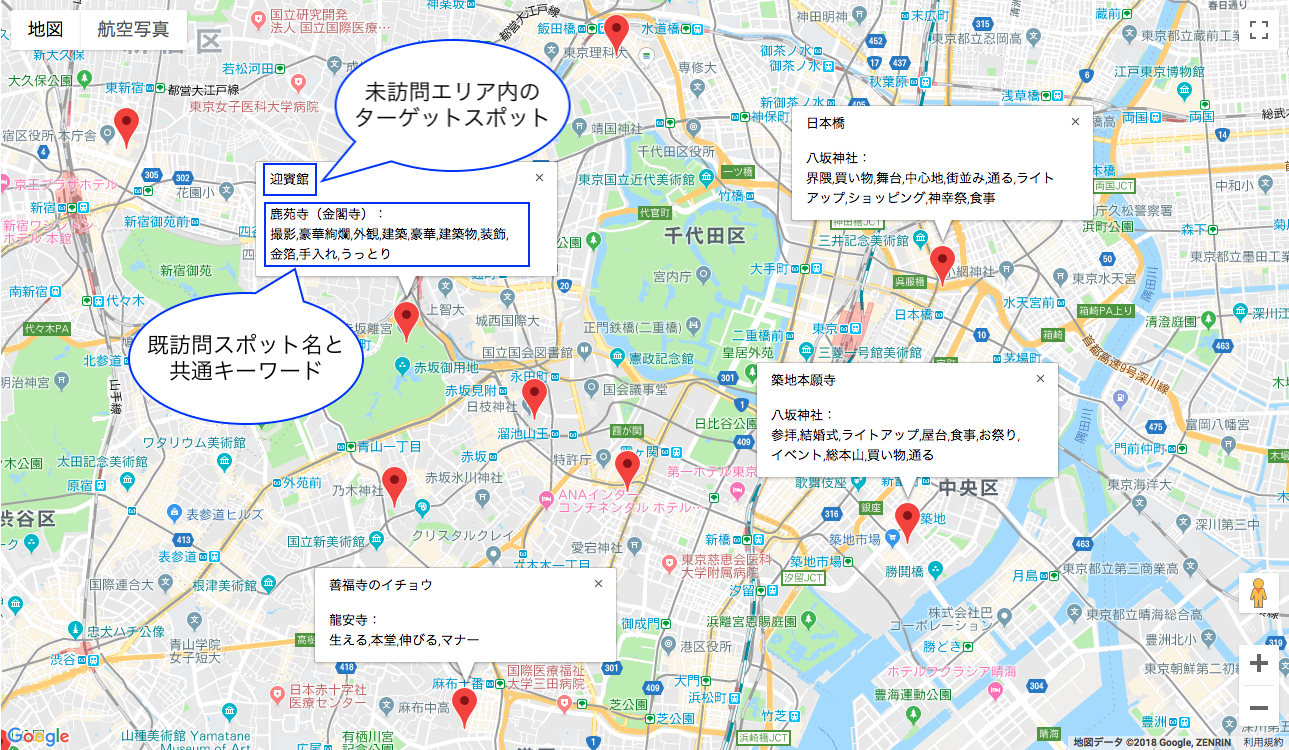
\includegraphics[clip,width=7.5cm]{picture/Photo_Map2_jap.png}
    \caption{プロトタイプシステム}
    \label{fig:Photo_Map}
   \end{center}
\end{figure}

%%%%%%%%%%%%%%%%%%%%%%%%%%%%%%%%%%%%%%%%%%
%%%%%%%%%%%%%%%%%%%%%%%%%%%%%%%%%%%%%%%%%
\section{関連研究}
ユーザの体験履歴を利用した検索や推薦システムに関する研究は数多く発表されている.
倉島ら\cite{Codd03}は,Flickrに投稿された写真のジオタグ情報を人々の旅行履歴として利用した旅行ルート推薦手法を提案した.
この手法では,ユーザの現在地から行きやすい場所とユーザの興味に合致した場所に移動しやすいと仮定し,行動モデルを生成している.
ユーザのジオタグ付き写真集合は,時間情報でソートすると個人の旅行履歴とみなすことができると考え,ジオタグ情報を利用してユーザの行動モデルを生成している.
北村らは\cite{Codd04},一般的な物体認識を用いて,過去の個人旅行写真から推定したユーザの旅行の嗜好に基づき観光地を推薦する方法を提案した.
物体認識システムを用いて,写真で撮った被写体情報のキーワードを取得し,グラフ視覚化技術によってキーワードの共起を表現した.
また,グラフの視覚化技術に基づいて旅行写真付きのグラフを視覚化するユーザインターフェイスを紹介した.
Chengらは\cite{Codd05},自由に利用できるコミュニティ投稿の写真を活用して,パーソナライズされた旅行のおすすめに焦点を当て,特定のユーザプロファイルまたは属性を考慮し,パーソナライズされた旅行の推奨を行うことを提案した.
観光地検索するとき,松本ら\cite{Codd08}はクチコミから特徴語を抽出して利用する研究を行なった.抽出対象を任意の名詞として,4種類の手法,TFIDF,ATF(Average Term Frequency),ポアソン確率,エントロピーのうちどの手法が特徴語抽出に適しているのか検討を行なった.また,抽出した特徴語を利用した検索支援システムを試作し,実験を通して特徴語提示の効果を検証した.
上原ら\cite{Codd09}はWebから観光情報を抽出し,複数の特徴ベクトルから観光地間の類似性を評価することで,観光地を推薦するシステムを提案した.観光地の特徴ベクトルは,知恵袋・ブログ上での共起キーワードと時系列分布,知恵袋上でのカテゴリ構造,観光地周辺施設,地図画像から生成した.これらの特徴ベクトルから観光地間の類似度の測定を行い,類似度の高い観光地を推薦した.

%%%%%%%%%%%%%%%%%%%%%%%%%%%%%%%%%%%%%%%%%%
%%%%%%%%%%%%%%%%%%%%%%%%%%%%%%%%%%%%%%%%%%
\section{未訪問スポットと既訪問スポットの対応付け}
\label{sec:未訪問スポットと既訪問スポットの対応付け}

我々は,未訪問スポットを理解しやすくするために,もっとも位置付けの近いユーザの既訪問スポットを対応付ける手法を提案する.
まず,ユーザが既に訪問した複数個の観光スポットとこれから訪問したい観光スポットエリア情報を入力する.
本手法では,観光スポットのユーザレビューを用いて特徴ベクトルを生成する.
さらに,ユーザの観光地の位置付けを抽出するために,あるスポットに対し他の訪れたスポットと比較した相対的特徴ベクトルを算出する.
同様に,未訪問スポットもエリア内の各スポットの特徴ベクトルを求める.
また,未訪問エリアの各観光スポットの相対的特徴ベクトルを,そのエリアの他の観光スポットと比較して計算する.
次に,相対的特徴ベクトルの類似度によって既訪問スポットを未訪問スポットと対応付ける.
最後に,その関係性を説明するためのキーワードを抽出する.

%%%%%%%%%%%%%%%%%%%%%%%%%%%%%%%%%%%%%%%%%%
\subsection{スポットのユーザレビューを用いた相対的特徴ベクトル生成}
\label{subsec:スポットのレビューから相対的特徴ベクトル生成}
本稿では,2016年9月末までのじゃらんから得られたレビューデータを使用する.
分散表現\cite{Codd06}を用いて観光スポットの特徴ベクトルの作成する.
このとき,観光スポット毎のレビューをまとめて1つの文書として扱う.
本研究では,分散表現を計算するためにPythonのライブラリであるgensim\footnote{https://radimrehurek.com/gensim/models/doc2vec.html}を利用する.
学習方法として,Distributed Bag-of-Wordsを利用して,各スポットの全レビューを使って300次元で作成したベクトルを使う.
既訪問スポットや未訪問スポットのレビューベクトルは,形態素解析器であるMeCab\cite{Codd07}に辞書「mecab-ipadic-NEologd」\footnote{https://github.com/neologd/mecab-ipadic-neologd/}用いて,分かち書き(原型)したレビューを利用して作成する.

各々の観光スポットは,ユーザによって,塩の強調するべき特徴は変化する.
たとえば,日本の有名な観光スポットを履歴に持つユーザにとっての「東京都庁舎展望台」と「金閣寺」について考える.
このとき,「金閣寺」の相対的特徴は,お寺,金色,京都などである.
一方,「東京都庁舎展望台」の相対的特徴は,展望,夜景,建物,新宿などが考えられる.
% さまざまな観光スポットと比較すると,相対的特徴は一般的な特徴,カテゴリ,場所になる傾向がある.

京都の寺院を履歴に持つユーザにとっての「金閣寺」と「清水寺」について考える.
このとき,同じ「金閣寺」でもお寺や京都などは特徴にはならず,「金閣寺」の相対的特徴は,金色,金箔,輝きなどとなる.
一方,「清水寺」の相対的特徴は,舞台や一望などである.
% どちらも京都にある寺院であるため,京都や寺院に関連する特徴は相対的特徴にならない.
% その代わりに,より詳細な特徴が相対的特徴として得られる.

相対的特徴ベクトル$r_{state,i}$を,式\ref{math:Vector difference}として定義する.
\begin{equation}
  r_{state,i}=s_i-average(S_{state}-s_i)
  \label{math:Vector difference}
\end{equation}
相対的特徴ベクトルは,そのスポット自体の特徴ベクトルから他のスポットの特徴ベクトルの平均を引いた値によって得られる.
$S_{state} =\{s_1,s_2,\dots,s_n\}$は,既訪問スポット集合もしくは未訪問スポット集合である.
$state$が$f$であれば,既訪問スポット集合を意味し,$state$が$u$であれば,未訪問スポット集合を意味する.
$s_i$は集合$S_{state}$内の観光スポット$i$の特徴ベクトルを示している.

%%%%%%%%%%%%%%%%%%%%%%%%%%%%%%%%%%%%%%%%%%
\subsection{対応するスポットの決定と特徴語の抽出}
\label{subsec:対応するスポットの決定と特徴語の抽出}
未訪問エリア内のスポットを既訪問スポットと対応付ける.
% そのため,未訪問スポットと既訪問スポットを,それらの相対的特徴ベクトルの類似度に基づいて対応付けを行う.
% 関連付け手順について説明する.
具体的には,ある未訪問スポットの相対的特徴ベクトルに最も類似度が高い既訪問スポットを対応付ける.
類似度計算には,コサイン尺度を用いる.
ただし,類似度が閾値(本研究では0.125)以下である場合は対応付けを行わない.

スポットの対応関係を示すだけでは,どのような点で対応するのかを理解するのは難しい.
そこで,未訪問スポットと既訪問スポットの関係性を表すキーワードをユーザに提示する.
しかし,分散表現である相対的特徴ベクトルから単語の特徴を得ることはできないため,他の方法を用いて単語を抽出する.

すべてのレビューを\ref{subsec:スポットのレビューから相対的特徴ベクトル生成}節と同様に形態素解析器MeCabによって単語に分割する.
ただし,助詞,助動詞,連体詞,記号,ストップワードを削除している.

キーワード抽出手順について説明する.
まず,TFIDF法を使って対象となる既訪問スポットと未訪問スポットの特徴語とTFIDF値を求める.
IDF値を算出する集合は$S_{state}$を用いる.

2つのスポットに共通する特徴語のTFIDF値の調和平均を用いて,対応付けしたスポットの説明可能なキーワードとして抽出する.
各単語のスコアを式\ref{math:Harmonic Mean}によって定義する.
\begin{eqnarray}
  score(t,s_f,s_u) = \frac{2 \times tfidf(t,s_f) \times tfidf(t,s_u)}{tfidf(t,s_f) + tfidf(t,s_u)}
  \label{math:Harmonic Mean}
\end{eqnarray}

$tfidf(t,s_f)$と$tfidf(t,s_u)$は同じ単語に関する既訪問スポット$s_f$におけるTFIDF値と未訪問スポット$s_u$におけるTFIDF値を示している.
単語スコアの上位$N$個の単語を説明情報としてユーザに提示する.

\subsection{実行例}
\label{subsec:実行例}

\begin{table}[t]
  \caption{既訪問スポット集合と未訪問スポット集合}
  \label{table:既訪問スポット集合と未訪問スポット集合}
  \centering
  \begin{tabular}{l|l}
  \hline
  \multicolumn{1}{c|}{既訪問スポット名} & \multicolumn{1}{c}{未訪問スポット名} \\ \hline
  浅草寺                           & 東京ディズニーランド(R)                \\
  小田原城址公園                       & 新宿御苑                         \\
  伏見稲荷大社                        & 東京スカイツリー                     \\
  奈良公園                          & 東京タワー大展望台                    \\
  三島スカイウォーク                     & 明治神宮                         \\ \hline
  \end{tabular}
\end{table}

\begin{table*}[t]
  \caption{説明情報の例}
  \label{table:説明情報の例}
  \centering
  \begin{tabular}{l|l|l}
  \hline
  \multicolumn{1}{c|}{未訪問スポット} & \multicolumn{1}{c|}{既訪問スポット} & \multicolumn{1}{c}{説明情報}                     \\ \hline
  新宿御苑                      & 小田原城址公園                         & お花見,咲き誇る,園内,桜の時,のんびり,手入れ,自然,遊具,ツツジ          \\
  東京スカイツリー                     & 三島スカイウォーク                    & 富士山,揺れ,高所恐怖症,揺れる,天井,絶景,エレベーター,パノラマ,展望デッキ,昇る \\ \hline
  \end{tabular}
\end{table*}

表\ref{table:既訪問スポット集合と未訪問スポット集合}は,ユーザ既訪問スポット集合と未訪問スポットの集合の例を示している.
未訪問スポットは東京都内からランダムに選んだ5つのスポットである.
表\ref{table:説明情報の例}は,\ref{sec:未訪問スポットと既訪問スポットの対応付け}節で提案した方法を用いて説明可能な単語の結果を示している.

公園という特徴に注目すると,未訪問スポット集合の中で公園に最も近いスポットは「新宿御苑」であると考えられる.
既訪問スポット集合の中には,「小田原城址公園」と「奈良公園」の2つの公園がある.
「小田原城址公園」には花や遊具に対する記述が多く,「奈良公園」には鹿や草に対する記述が多い.
「新宿御苑」には花や遊具に対する記述が多いため,「小田原城址公園」との関係性があると考えられる.

「三島スカイウォーク」は既訪問スポット集合の中で眺めがいい,高いの特徴が最も強いことが考えられる.
一方,未訪問スポット集合の中で眺めがいい,高いの特徴が強いのは「東京スカイツリー」や「東京タワー大展望台」の2つがある.
このとき,どちらも正しい回答だと考えられる.
この例では,「東京スカイツリー」はより見やすいと考えられるため関連付けされる.
また,説明キーワードとして「富士山」が抽出される.
良い景色を強調する言葉として一般的であり,これによって関係を適切に表現している.
提案手法の方は各関係の特徴を示すことができる.

%%%%%%%%%%%%%%%%%%%%%%%%%%%%%%%%%%%%%%%%%%
%%%%%%%%%%%%%%%%%%%%%%%%%%%%%%%%%%%%%%%%%%
\section{対応関係を表す特徴語抽出の評価}
\label{sec:対応関係を表す特徴語抽出の評価}
%%%%%%%%%%%%%%%%%%%%%%%%%%%%%%%%%%%%%%%%%%
\subsection{実験内容}
提案手法の特徴語抽出について評価を行うため,他のキーワード抽出手法と比較して評価を行う.
以下の3つの方法を使って比較する.
\begin{description}
  \item A.算術平均
  \item B.乗算
  \item C.提案手法(調和平均)
\end{description}

\begin{table}[t]
  \caption{対応関係を表す特徴語の実験結果}
  \label{table:対応関係を表す特徴語の実験結果}
  \centering
  \begin{tabular}{c|r|r|r}
  \hline
  評価 & \multicolumn{1}{c|}{算術平均} & \multicolumn{1}{c|}{乗算} & \multicolumn{1}{c}{提案手法} \\ \hline
  1  & 28.28\%                  & 31.31\%                  & 29.29\%                 \\
  2  & 35.35\%                  & 31.31\%                  & 35.35\%                 \\
  3  & 10.10\%                   & 14.14\%                  & 12.12\%                 \\
  4  & 26.26\%                  & 23.23\%                  & 23.23\%                 \\ \hline
  \end{tabular}
\end{table}

% 方法Aと方法Bは,まず,各スポットの特徴として\ref{subsec:スポットのレビューから特徴ベクトル生成}節で作成された特徴ベクトルを使用する.
% そして,\ref{subsec:対応するスポットの決定と特徴語の抽出}節を用いて既訪問スポットと未訪問スポットの特徴語とTFIDF値を求める.

キーワードを抽出するとき,方法Aでは,2つのスポットに共通する特徴語のスコアとして算術平均を計算する.抽出した単語のスコアを式\ref{math:Mean}によって定義する.
\begin{eqnarray}
  score(t,s_f,s_u) = \frac{tfidf(t,s_f) + tfidf(t,s_u)}{2}
  \label{math:Mean}
\end{eqnarray}

方法Bでは,2つのスポットに共通する特徴語のスコアとして乗算を計算する.抽出した単語のスコアを式\ref{math:Multi}によって定義する.
\begin{eqnarray}
  score(t,s_f,s_u) = tfidf(t,s_f) \times tfidf(t,s_u)
  \label{math:Multi}
\end{eqnarray}

% 式\ref{math:Mean},式\ref{math:Multi}の$TFIDF(t,d,f)$と$TFIDF(t,d,u)$は同じ単語に関する既訪問スポットのTFIDF値と未訪問スポットのTFIDF値を示している.単語スコアの上位$N$個の単語を説明情報としてユーザに提示する.

%%%%%%%%%%%%%%%%%%%%%%%%%%%%%%%%%%%%%%%%%%
\subsection{実験手順}
\label{subsec:実験手順}
クラウドソーシングのサービスである,CrowdWorks\footnote{https://crowdworks.jp/}を利用して23人の被験者を集めた.
% 各方法を用いて,被験者の既訪問スポットに基づいて,未訪問スポットの説明可能な情報を提示した.
まず,被験者は4から10個の自分が既に訪れたことのある観光スポットを入力した.
% 本実験では,入力文字列とシステム内のスポット名を照会するために,入力文字列から検索したスポット名候補の中から対象スポットを選択した.
次に,被験者は旅行などで行ったことがなく,これから訪れたい都道府県やエリアを入力した.

本手法では,方法AからCそれぞれにおいて,対応付けられた既訪問スポットと未訪問スポット,およびスポット同士の関係を説明する特徴語を最大で5つまで提示した.
結果を評価するために,被験者は以下の4つの選択肢から1つを選んだ.
\begin{enumerate}
  \item 2つのスポットには関係性があり,キーワード\footnote{関係を説明する特徴語のことであるが,被験者には単にキーワードと示した.}によって関係が明確になった.
  \item 2つのスポットの関係性があり,キーワードによって初めて気がついた.
  \item 2つのスポットには関係性があるが,キーワードは関係を表していない.
  \item 2つのスポットには関係性がない.
\end{enumerate}
%%%%%%%%%%%%%%%%%%%%%%%%%%%%%%%%%%%%%%%%%%
\subsection{実験結果と考察}
表\ref{table:対応関係を表す特徴語の実験結果}は,方法AからCにおける選択肢1から4それぞれの選択割合を示している.
方法Bでは,多くの被験者が選択肢1を選択している.
このことから,方法Bは明らかな関係を表現する特徴語抽出ができることがわかった.
方法AとCでは,選択肢1の割合が減少し,選択肢2の割合が増加している.
このことから,方法AとCは隠れた関係を表現する特徴語を見つけて被験者に提示することができると考えた.
しかし,方法Aでは,選択肢4の割合が増加しているため,方法Cより無関係な特徴語を抽出しやすくなったといえる.
また,選択肢1と2を合計すると,方法Cが最も高くなった.
このことから,説明するためのスポットの関連を説明する特徴語としては方法Cが妥当といえる.

%%%%%%%%%%%%%%%%%%%%%%%%%%%%%%%%%%%%%%%%%%
%%%%%%%%%%%%%%%%%%%%%%%%%%%%%%%%%%%%%%%%%%
\section{対応付けに関する評価}
\label{sec:対応付けに関する評価}
%%%%%%%%%%%%%%%%%%%%%%%%%%%%%%%%%%%%%%%%%%
\subsection{実験内容}
特徴語抽出については\ref{subsec:対応するスポットの決定と特徴語の抽出}節の手法を用いる.
提案手法を対応付け方法について,以下の3つの手法を比較して評価を行う.
\begin{description}
  \item D.メタデータの一致度(カテゴリ,滞在時間,訪問時期)
  \item E.分散表現の類似度(特徴ベクトル)
  \item C.提案手法(相対的特徴ベクトル)
\end{description}

方法Dは,観光スポット検索サイトでスポットを検索するためのメタデータである.
次のように,検索によく使われる3つのメタデータを選択する.
\begin{itemize}
 \item カテゴリ:神社・神宮・寺院,観光施設・名所巡り等
 \item 滞在時間:1時間未満,1--2時間等
 \item 訪問時期:1--12月,春,夏,秋,冬
\end{itemize}

方法Dでは,カテゴリ,滞在時間,季節が一致する既訪問スポットと未訪問スポットを抽出する.
抽出できない場合は,季節,滞在時間,カテゴリの順に条件を緩和する.
既訪問スポットが複数ある場合は,レビュー数が最も多いスポットを選択する.

方法Eでは,各スポットの特徴として\ref{subsec:スポットのレビューから相対的特徴ベクトル生成}節で作成した特徴ベクトルを使用する.
すなわち,式\ref{math:Vector difference}を用いずに,レビューから得た分散表現をそのまま用いる.

クラウドソーシングのサービスである,CrowdWorksを利用して24人の被験者を集めた.
実験手順は\ref{subsec:実験手順}節で説明した手順と同じである.

%%%%%%%%%%%%%%%%%%%%%%%%%%%%%%%%%%%%%%%%%%
\subsection{実験結果と考察}

\begin{table}[t]
  \caption{対応付けに関する実験結果}
  \label{table:対応付けに関する実験結果}
  \centering
  \begin{tabular}{c|r|r|r}
  \hline
  評価 & \multicolumn{1}{c|}{メタデータ} & \multicolumn{1}{c|}{分散表現} & \multicolumn{1}{c}{提案手法} \\ \hline
  1  & 41.30\%                    & 33.85\%                    & 29.36\% \\
  2  & 43.48\%                    & 47.69\%                    & 48.62\% \\
  3  & 2.17\%                     & 2.31\%                     & 2.75\% \\
  4  & 13.04\%                    & 16.15\%                    & 19.27\% \\
  \hline
  対応付け数  & 46                    & 130                    & 109 \\
   \hline
  \end{tabular}
\end{table}

対応付けしたスポットの合計数は285である.
表\ref{table:対応付けに関する実験結果}は,それぞれの方法における選択肢1から5それぞれの選択割合を示している.
方法Dについて,多くの被験者が選択肢2を選択している.
このことから,方法Dは明らかな関係にあるスポット同士を関連付けることができることがわかった.
他の方法と比較して,方法C(提案手法)では,選択肢1の割合が減少し,選択肢2の割合が増加している.
このことから,方法Cは隠れた関係を見つけて被験者に提示することができると考えた.
しかし,選択肢4の割合も増加しているため,無関係なスポットを抽出しやすくなったといえる.

選択肢1と2を合計すると,方法Dが最も高くなる.
このことから,説明するためのスポットの対応付けの精度が最も高いといえる.
しかし,方法Dは対応付けすることができるスポットの数が他の手法に比べ半分以下であり,未訪問スポットの多くに説明を付与することができない.

方法Eと方法Cを詳細に考察するために,既訪問スポットの入力別に分析した.
% 被験者が入力した既訪問スポットのカテゴリが異なる場合は同様の傾向を示した.
入力した既訪問スポットの半数以上が同一カテゴリのスポットであった被験者(表中の同じ場合)とそうではない被験者(表中の異なる場合)に分けて集計した.
表\ref{table:対応付けしたスポット中}は選択肢1と選択肢2の評価の割合である.
提案手法である方法Cを使用すると,カテゴリが異なる場合において,方法Eよりも1よとび2の割合を増加させることができる.
相対的特徴ベクトルを用いることによって,カテゴリをこえて各スポットの特徴を求めることができるといえる.
% 既訪問スポットのジャンルが類似する場合では,方法Eの方がより良い評価となっている.
カテゴリが同じ場合の選択肢1は方法Cでは,少なくなっている.
これは,相対的特徴ベクトルとしては,カテゴリの特徴が打ち消されたベクトルが生成されるため,明らかな関係となる対応付けが減ったと考えられる.
しかし,選択肢2が増えずに4が増え,無関係に見える対応付けを増やす結果となった.
入力スポットの種類によって対応付け手法を切り変えることが有効と考えられる.

\begin{table}[t]
  \caption{対応付けしたスポット中の既訪問スポットのカテゴリが異なる場合と同じ場合の評価割合}
  \label{table:対応付けしたスポット中}
  \centering
  \begin{tabular}{c|c|r|r}
  \hline
  &     & \multicolumn{1}{c|}{分散表現} & \multicolumn{1}{c}{提案手法} \\ \hline
  異なる場合                 & 評価1 & 19.23\%                  & 21.10\%                 \\ \cline{2-4}
  & 評価2 & 24.62\%                  & 25.69\%                 \\ \hline
  同じ場合                  & 評価1 & 14.62\%                  & 8.26\%                  \\ \cline{2-4}
  \multicolumn{1}{l|}{} & 評価2 & 23.08\%                  & 22.94\%                 \\ \hline
  \end{tabular}
\end{table}

%%%%%%%%%%%%%%%%%%%%%%%%%%%%%%%%%%%%%%%%%%
%%%%%%%%%%%%%%%%%%%%%%%%%%%%%%%%%%%%%%%%%%
\section{未訪問スポット説明の有効性評価}
\label{sec:未訪問スポット説明の有効性評価}
%%%%%%%%%%%%%%%%%%%%%%%%%%%%%%%%%%%%%%%%%%
\subsection{実験内容}
提案手法の有効性を評価するために以下の2つのシステムを使って比較する.
\begin{description}
  \item a.未訪問スポット名のみを表示
  \item b.未訪問スポット名,対応する入力スポット,対応を説明する特徴語を表示(提案手法)
\end{description}

被験者の入力は,これまでの実験と同様に,4個から10個の自分が既に訪れたことのある観光スポットと訪問したいエリアである.
ただし,エリアは2つ入力し,それぞれ別々にシステムa,システムbの入力として用いた.
なそ,システムaとシステムbはランダムな順番で実行される.
システムを評価するために,被験者は以下の2つの設問について回答した.
また,それらの選択理由について自由記述で答えた.

\begin{description}
  \item Q1. 表示されたスポットの詳細情報はどちらの方が分かりやすいかを選択してください.
  \item Q2. 旅行の計画を立てる際にどちらの方が使いたいかを選択してください.
\end{description}

\subsection{実験結果と考察}
Q1に対する回答について,システムaとシステムbの結果はそれぞれ12件と38件となった.
被験者の回答理由の例を表\ref{table:被験者がシステムaの方が良いと回答した例}(システムa)および,表\ref{table:被験者がシステムbの方が良いと回答した例}(システムb)に示す.
また,
旅行の計画を立てる際にどちらの方が使いたいかに対する回答について,システムaとシステムbの結果はそれぞれ10件と40件となった.
被験者の回答より,得られた2つのシステムの特徴をまとめる.

システムbでは,キーワードや関連している情報が表示されており分かりやすいという特徴がある.
これに対し,システムaでは,スポット名のみが表示されているためシンプルで分かりやすいという特徴があるが,なぜそのスポットが検索されたのか分からないなどの否定的な回答も多数あった.
システムの表示情報が「シンプルな方が良い」と「詳細な情報が良い」の2つに大きく分けられているが,Q2の回答より80\%の被験者はシステムbの方が使いたいと回答しており,提案手法の方が評価が高いといえる.
また,システムbに関してスポットの写真を載せるとより分かりやすいなどの意見があり,画像による関連性の説明という拡張が考えられる.

\begin{table}[t]
  \caption{被験者がシステムaの方が良いと回答した例}
  \label{table:被験者がシステムaの方が良いと回答した例}
  \centering
  \begin{tabular}{l}
  \hline
  \begin{tabular}[c]{@{}l@{}}スポット名だけ書いてあるのでごちゃごちゃにならず、一目でどこに\\ 何があるか分かるからです.\end{tabular} \\ \hline
  スポットだけ表示されるところがシンプルで分かりやすかったから.                                                         \\ \hline
  シンプルにそのエリアの観光スポットを知ることが出来る.                                                             \\ \hline
  \end{tabular}
\end{table}

\begin{table}[t]
  \caption{被験者がシステムbの方が良いと回答した例}
  \label{table:被験者がシステムbの方が良いと回答した例}
  \centering
  \begin{tabular}{l}
  \hline
  自分が訪れた事のあるスポットと関連性があり連想しやすいから.                                                 \\ \hline
  \begin{tabular}[c]{@{}l@{}}どのような場所か想像しやすいので、計画を立てるのにも使いたい\\ と思ったから.\end{tabular} \\ \hline
  何と関連して表示された等詳細の情報が表示されわかりやすかった.                                                  \\ \hline
  \end{tabular}
\end{table}

%%%%%%%%%%%%%%%%%%%%%%%%%%%%%%%%%%%%%%%%%%
%%%%%%%%%%%%%%%%%%%%%%%%%%%%%%%%%%%%%%%%%%
\section{まとめと今後の課題}
\label{sec:まとめと今後の課題}

本研究では,ユーザが行きたい観光スポットが決まっていない場合に,ユーザの事前知識が不足しているため,観光検索サイトを使用してランキング,おすすめ情報やカテゴリなどを基に検索された観光スポットに対する理解が困難であることに着目した.
未訪問スポットに対する理解を支援するために,未訪問スポットをユーザが既に訪れたことがある既訪問スポットと比較することによって,理解を支援する説明手法を提案した.

キーワードの抽出の評価について,提案手法の方が既訪問スポットによる未訪問スポットの説明性が高いことを確認した.
対応付け手法の結果として,メタデータの一致に基づく手法では,未訪問スポットと対応付けできる既訪問スポットが最も少なくなることがわかった.
相対的特徴ベクトルと調和平均を利用することによって,各スポットの特徴を求めることができた.
また,未訪問スポットと既訪問スポットに対して意外性がある関連付けが可能で,ユーザが知らない観光スポットに対する興味と関心を集めることができる可能性があることを確認した.
システム評価について,提案手法の方がより詳細な情報を提示しているため,ユーザが未訪問スポットをイメージしやすいことを確認した.

今後の課題としては,レビュー数が少ないスポットに対する関連付けの精度が低いため,新たな方法を検討する必要がある.また,ある観光スポットに類似する特徴を持つ既訪問スポットで説明するだけではなく,既訪問スポット集合と対象観光スポットの関係を説明可能な可視化インタフェースへと拡張する予定である.

%%%%%%%%%%%%%%%%%%%%%%%%%%%%%%%%%%%%%%%%%%
\begin{acknowledgment}
本研究の一部は,平成30年度科研費基盤研究(C)(課題番号:18K11551)によるものです.ここに記して謝意を表すものとします.
\end{acknowledgment}


%%%%%%%%%%%%%%%%%%%%%%%%%%%%%%%%%%%%%%%%%%
\begin{thebibliography}{11}
  \bibitem{Codd01}
    D. Gentner,
      ``Structure-Mapping: A Theoretical Framework for Analogy'',
      Cognitive Science, Vol.7, pp.155–170, 1983
  \bibitem{Codd02}
    K. J. Holyoak and P. Thagard,
      ``Analogical Mapping by Constraint Satisfaction'',
      Cognitive Science, Vol.13, pp.295–355, 1989
  \bibitem{Codd03}
    T. Kurashima, T. Iwata, G. Irie and K. Fujimura.,
      ``Travel route recommendation using geotags in photo sharing sites'',
      CIKM '10 Proceedings of the 19th ACM international conference on Information and knowledge management, pp.579-588, 2010
  \bibitem{Codd04}
    R. Kitamura and T. Itoh,
      ``Tourist Spot Recommmendation Applying Generic Object Recognition with Travel Photos'',
      ITE Tech. Rep., Vol.42, No.12, AIT2018-94, pp.185-188, 2018
  \bibitem{Codd05}
    A. J. Cheng, Y. Y. Chen, Y. T. Huang and Winston H. Hsu,
      ``Personalized Travel Recommendation by Mining People Attributes from Community-Contributed Photos'',
      MM '11 Proceedings of the 19th ACM international conference on Multimedia, pp.83-92, 2011
  \bibitem{Codd06}
    Quoc V. Le and Tomas Mikolov,
      ``Distributed representations of sentences and documents'',
      In Proceedings of the 31th International Conference on Machine Learning, ICML 2014, pp. 1188–1196, 2014
  \bibitem{Codd07}
    T. Kudo, K. Yamamoto and Y. Matsumoto,
      ``Applying Conditional Random Fields to Japanese Morphological Analysis'',
      Proceedings of the 2004 Conference on Empirical Methods in Natural Language Processing (EMNLP-2004), pp.230-237, 2004
  \bibitem{Codd08}
    松本 敦志, 杉本 徹,
      ``クチコミから抽出した特徴語を利用する観光地検索支援'',
      第75回全国大会講演論文集, Vol.2013, No.1, pp.307-308, 2013
  \bibitem{Codd09}
    上原 尚, 嶋田 和孝, 遠藤 勉,
      ``Web上に混在する観光情報を活用した観光地推薦システム'',
      社団法人 電子情報通信学会, 信学技報, Vol.112, No.367, pp.13-18, 2012
\end{thebibliography}

\begin{biography}
\profile{n}{潘 健太}{1996年生.2018年工学院大学情報学部コンピュータ科学科卒業.
2018年同大学大学院工学研究科情報専攻修士課程入学,現在に至る.観光スポット検索に興味を持つ.}
%
\profile{n}{北山 大輔}{2009年兵庫県立大学大学院環境人間学研究科博士後期課程修了.同年同学科客員研究員.2011同学科特任助教.2012年工学院大学情報学部助教.2016年同学部准教授,現在に至る.博士(環境人間学).Webマイニング,地理情報検索/推薦ベースを研究.電子情報通信学会.日本データベース学会各会員.}
\end{biography}

\end{document}
